\documentclass[12pt]{article}
\usepackage[utf8]{inputenc}
\title{\vspace{-2.75cm}Conflating Global Finance with Technological Competition: The U.S.'s Reaction to Chinese Foreign Aid\vspace{-0.5cm}}
\author{Nicholas Ray}
\date{\vspace{-0.30cm}November 14 2022\vspace{-1cm}}
\usepackage[margin=1in]{geometry}
\usepackage{mathtools,amssymb,amsthm}
\usepackage{setspace}
\doublespacing
\usepackage{footmisc}
\renewcommand{\footnotelayout}{\setstretch{1.75}}
\usepackage{footmisc}
\renewcommand{\footnotesize}{\normalsize}
\usepackage{caption}
\usepackage{tikz}
\usepackage{istgame}
\usepackage[backend=biber, style=authoryear, maxbibnames=99,uniquelist=false]{biblatex}
\renewbibmacro{in:}{}
\renewbibmacro*{volume+number+eid}{%
  \printfield{volume}
  \setunit*{\addnbthinspace}
  \printfield{number}
  \setunit{\addcomma\space}
  \printfield{eid}}
\DeclareFieldFormat[article]{number}{\mkbibparens{#1}}
\AtEveryBibitem{
  \clearfield{issn}
  \clearfield{month}
  \clearfield{urlyear}
  \clearlist{language}
  \clearfield{note}
  \clearfield{month}
  \clearfield{day}
  \ifentrytype{online}{}{
    \clearfield{url}
  }
}
\addbibresource{ForeignAidBib.bib}
\begin{document}
\maketitle
\begin{abstract}
    The U.S. and China appear to be at variance on the global finance stage and locked in a technological arms race. While recent studies on foreign aid have focused on how China's aid programs have changed the conditionality and effectiveness of Western aid, I instead seek to understand how the U.S. may have changed its foreign aid strategy in response to competition from China along the dimension of technology and the internet. I argue that it is rational for the U.S. to react to Chinese aid by conditioning its aid on a recipient's use of the internet in an effort to combat China's suspected negative influence. I find that a measure for internet governance and Chinese aid are statistically significant predictors for U.S. foreign aid in a sample of 44 African countries between 2010 and 2017. 
\end{abstract}

\section*{Introduction}
Research on foreign aid has seemingly concluded that donors use aid as a self-interested policy tool (e.g., \cite{alesina2000}; \cite{hoeffler2011}) and that its effectiveness greatly varies (e.g., see \cite{christensen2011}).\footnote{All data and code can be found on GitHub at https://github.com/nnray/Analysis. In the ``Code'' folder, navigate to ``628.Rmd'' for my R script. My full \LaTeX \;file can be found at https://github.com/nnray/628 under ``RoughDraft.tex''.} Contemporary foreign aid work has largely sought to understand how the recent influx of aid from the People's Republic of China (China) has affected these conclusions. There is some evidence that traditional, Western donors have updated how they give aid and that aid effectiveness itself has changed. For example, albeit with loans, the World Bank appears to have reduced the conditions it places on borrowing countries (\cite{hernandez2017}) while aid from the United States (U.S.) seems to have become more effective at stimulating liberal democratic values (\cite{blair2022}).

Thus far, this literature has overlooked a potentially salient factor for how Western donors allocate aid in a world increasingly exposed to Chinese finance: the internet. China is thought to be exporting technology alongside its aid programs in a bid to spread its influence and stimulate domestic economic growth, although countries like the U.S. accuse China of promoting so-called ``digital authoritarianism'' (\cite{u.s.departmentofstate2010}; \cite{u.s.departmentofstate2022}). The U.S., by contrast, prefers a politically and economically liberal internet where governments invoke the principle of ``laissez faire.'' While seemingly trivial, this viewpoint of the U.S. reflects the increasing competition between the two countries for technological superiority (\cite{hassetal.2021}). 

How then has the U.S. reacted to an increase in Chinese aid spending around the world, given that China is also a rival on this separate dimension of technology and the internet? More pointedly, is the U.S. allocating foreign aid in a way that enables it to compete with China technologically? I claim that this makes sense given the foreign policy emphasis the U.S. has placed on the world-wide internet and the contemporary effectiveness U.S. aid has had on liberal values. The U.S., by countering aid programs from China that it suspects might negatively affect recipient's model of the internet, can prevent the erosion of internet liberalism in a country.

If this were true, it would be a contribution to both the foreign aid literature and the burgeoning area of work dedicated to understanding China's influence on the liberal international order (LIO). Where current work on the LIO focus on how China may or may not be a threat to the pillars of economic or political liberalism (e.g., \cite{weiss}; \cite{broz}), this article can speak to how China is potentially influencing the LIO's similar upholding of internet liberalism. China may undermine this tenet, although unintentionally so as a by-product of sharing its technology for economic reasons.

I proceed as follows. In the next section, I present my argument and theoretical reasoning for why the U.S. might be expected to alter its foreign aid spending in response to the recent spending by China. After developing implications and hypotheses, I describe my empirical strategy and data. Results and a discussion of the findings are presented before concluding.

\section*{Theory}
\subsection*{Model}
I argue that it is rational for the U.S. to consider the internet when distributing foreign aid and, specifically, that a recipient's current use of the internet should be a strong predictor for receiving U.S. funds. To explore the rationality of this alleged behavior, I consider a simple entry deterrence game. China is the first-mover and decides to enter or spend foreign aid in a particular country by allocating aid or not. The U.S. then moves second, making a similar decision to distribute foreign aid depending on if China has entered or not. There are two parameters that decide the payoffs of the game: $\gamma$, the influence that Chinese aid has on a recipient country's internet model and $\delta$, the influence of U.S. aid. Low values represent high degrees of influence for both. Essentially, the strategies of the players are symmetrical, with each country deciding to spend aid if their degree of influence is relatively larger than their rival's.

When U.S. foreign aid is net effective at encouraging a liberal model of the internet in a country, it decides to allocate aid. China, observing the U.S.'s expenditure, decides not to distribute foreign aid in that country. However, if the U.S. concludes not to spend aid monies due to its aid being relatively ineffective at influencing a recipient's use of the internet, then China allocates aid and exerts its influence on a recipient's internet usage. The extensive-form of this game is displayed in Figure 1, with more detail given in the appendix.

\subsubsection*{Figure 1}
\begin{istgame}[scale=4]
\xtdistance{5mm}{15mm}
\istroot(0)(0,0){\textit{China}}
\istb{\neg Spend}[al]
\istb{Spend}[ar]{0\leq\gamma,c,\delta\leq1}[below,yshift=25mm,xshift=25mm]
\endist
\xtdistance{5mm}{10mm}
\istroot(1)(0-1)<above left>{\textit{U.S.}}
\istb{\neg Spend}[l]{(\gamma,\;\delta)}
\istb{Spend}[r]{(\gamma,\;\frac{1}{\delta}-c_2)}
\endist
\istroot(2)(0-2)<above right>{\textit{U.S.}}
\istb{\neg Spend}[l]{(\frac{1}{\gamma}-c_1,\;\delta)}
\istb{Spend}[r]{(\frac{\delta}{\gamma}-c_1,\;\frac{\gamma}{\delta}-c_2)}
\endist
\xtdistance{10mm}{10mm}
\end{istgame}

\subsection*{Notable Assumptions}
Ample explanation is in order. Firstly, there is a host of technical restrictions inherent to my argument. Other determinants of foreign aid, for example, are not considered here. Thus, any changes in spending should be interpreted as the U.S. or China deciding to spend on internet influence or not $ceteris\;paribus$, or holding other foreign aid avenues constant. 

These decisions are also stipulated as dichotomous, where China or the U.S. simply agree to spend foreign aid or not. In reality, foreign aid spending is clearly continuous in nature and, moreover, typically based on repeated interactions between both other donors and recipients. This is also a full information model, with no uncertainty present over players' decisions to spend. I further assume that payoffs from the decision to spend or not are zero-sum at the extremes, where an arbitrarily large influence by one country dwarfs the incentives for the other to spend foreign aid.

Secondly, and most critically, there are a number of substantive assumptions invoked in this theoretical exposition that must be detailed. For one, I am assuming that the U.S. has a preference over internet governance around the world and, additionally, that foreign aid is an effective instrument for the U.S. to actualize this preference. Somewhat symmetrically, I assume that Chinese aid has an effect on a recipient's internet model and that this effect is negative or illiberal. I will take these assumptions in turn, connecting these behavioral claims to the established literature where possible.

Beginning with the U.S., there is suggestive evidence that the U.S. has a preference over how other countries use the internet. In 2022, bipartisan legislation was introduced in the Senate to increase funding to so-called ``internet freedom programs'' (\cite{foreignrelationscommittee2022}), which were started by the U.S. Department of State in the 2000's to combat censorship and surveillance in other countries (\cite{u.s.departmentofstate2021}; \cite{hanson2012}). Also in 2022, a declaration was led by the U.S. and signed by over 60 other countries to combat global ``digital authoritarianism'' (\cite{u.s.departmentofstate2022}). These concerns stretch back to at least 2010, when then-Secretary of State Hillary Clinton (\cite{u.s.departmentofstate2010}) stated the U.S. desired a free internet around the world.

If one accepts that the U.S.'s apparent foreign policy position on the internet coincides with more traditional accounts of U.S. preferences for democracy world-wide, then there is indirect evidence that foreign aid is an effective tool for influencing internet politics in recipient countries. For instance, in Africa U.S. aid is found to be relatively successful in promoting liberal democratic values amongst Afrobarometer respondents when compared to Chinese foreign aid \cite{blair2022}. There is also evidence that U.S. aid is most effective at achieving its goals in countries not currently receiving large amounts of Chinese aid (\cite{dreher2021}).

Turning to China, there is reason to believe that Chinese aid could influence a recipient's political use of the internet in an illiberal manner. China launched the Belt and Road Initiative (BRI) in 2013 and the Digital Silk Road (DSR) in 2015, both aimed at enlarging China's global influence while strengthening economic growth (\cite{dreher2022}). In doing so, it is alleged that China is sharing technology with recipient states that could improve state capacity and allow recipients to curb free expression, both digitally and physically (\cite{hillman2021}). Other work, though, rightly points out that China is a non-unitary actor with private firms that could undermine a state-led technology sharing campaign (\cite{shen2018a}) and that China's technology spending has not changed much immediately following the announcement of the DSR (\cite{tugendhat2021}). 

However, it seems most pertinent to this study that the West believes China to be spreading its illiberal model of the internet (e.g., \cite{hillman2021}; \cite{u.s.departmentofstate2022}), or at least that there is a good chance for it to (\cite{triolo2020}). Further, there is evidence that Chinese foreign aid encourages feelings of acceptance towards autocratic leadership in African countries (\cite{gehring2022}).

\subsection*{Implications}
Returning to my theory, the model simplistically states that the U.S. and China should allocate foreign aid when aid is relatively effective at influencing a recipient's political model of the internet. Some of the literature implies that U.S. aid is effective when Chinese aid is low or not present (\cite{dreher2021}). Since it is assumed that Chinese aid has a negative effect on how recipients use the internet, this further implies that U.S. aid should be spent in countries with more liberal models of the internet to ensure maximum effectiveness. These concurrent implications lead to the following hypotheses:

\begin{align*}
    &\text{``Interstate Competition Hypothesis''}\\
    H_{1a}&:\;\text{U.S. aid inversely related to Chinese aid}\\
    &\text{``Trickle Down Hypothesis''}\\
    H_{2a}&:\;\text{U.S. aid directly related to recipient internet model}\\
\end{align*}

I label $H_{1a}$ the ``Interstate Competition Hypothesis'' because if U.S. foreign aid is truly most effective where Chinese aid is not present, this implies that the U.S. would respond to an increase in Chinese aid by focusing its spending in countries not currently receiving aid from China. China and the U.S. would thus be spending in completely separate countries or regions.

$H_{2a}$ is titled the ``Trickle Down Hypothesis'' since the U.S. would spend more foreign aid in countries with more liberal internet models, implying that the U.S.'s preference for a globally liberal internet model is manifested by it focusing on bolstering countries with already relatively liberal models.

However, it is also hypothetically possible that the U.S. would try to compete with Chinese aid by directly countering it in countries where the Chinese are active and generating intrastate competition. Similarly, it could make sense for the U.S. to be focusing on improving the internet in countries with relatively illiberal models, as it is plausible that foreign aid's influence on the internet would have higher marginal benefits. This opposing set of logic generates the following hypotheses:
\begin{align*}
    &\text{``Intrastate Competition Hypothesis''}\\
    H_{1b}&:\;\text{U.S. aid directly related to Chinese aid}\\
    &\text{``Bottom Up Hypothesis''}\\
    H_{2b}&:\;\text{U.S. aid inversely related to recipient internet model}\\
\end{align*}

\section*{Empirics}
\subsection*{Setting}
I test these hypotheses by evaluating the relationship between U.S. aid, Chinese aid, and the internet across 44 African countries between 2010 and 2017. The full set of countries includes: Algeria, Angola, Benin, Botswana, Burundi, Cabo Verde, Cameroon, Central African Republic, Chad, Comoros, Republic of the Congo, Cote d'Ivoire, Democratic Republic of the Congo, Djibouti, Egypt, Equatorial Guinea, Ethiopia, Gabon, Gambia, Ghana, Guinea, Guinea-Bissau, Kenya, Lesotho, Liberia, Madagascar, Malawi, Mali, Mauritania, Mauritius, Morocco, Mozambique, Namibia, Niger, Nigeria, Rwanda, Senegal, Sierra Leone, South Africa, Togo, Tunisia, Uganda, Zambia, and Zimbabwe. 

I chose to focus on Africa during this time period for three main reasons. Firstly, Africa has been a major area of focus for China's finance projects, with the Council on Foreign Relations claiming that ``China already provides more financing for information and communications technology than all multilateral agencies and leading democracies combined do across the continent'' (\cite{kurlantzicketal.2020}). Secondly, the data I use for Chinese spending ends in 2017. Thirdly, while 2010 is indeed an arbitrary starting point, it seems like a reasonable choice since both Chinese aid and the internet diminish greatly before this period.

\subsection*{Data and Variables}
%internet freedom
In operationalizing my theory, I measure the political use of the internet as ``internet freedom'' from the Digital Society Project (DSP). The DSP aims to identify ``how people use social media as a political tool and to explore how political institutions and social media use interact,'' providing data from expert surveys that cover a range of topics such as censorship, disinformation, and monitoring (\cite{mechkova2022}). The DSP employs methodology designed by the Varieties of Democracy project (V-Dem, \cite{coppedge2022}) to try and estimate differences in expert opinion and knowledge.

The DSP is one of two indices measuring a political concept of internet usage and data from the DSP is potentially superior for measuring the concept of internet liberalism in Africa compared to the primary alternative, Freedom on the Net (FOTN, \cite{freedomhouse2022}). FOTN frequently features missing data for the continent of Africa and does not take into account possible variations in expert opinion and knowledge like the DSP does.

%Chinese aid
The other main explanatory variable is Chinese foreign aid, stemming from the College of William \& Mary's AidData research lab (\cite{custer2021}). This is the one of the only datasets on Chinese aid and is certainly the largest and most specific. Aid is quantified as official financial and in-kind commitments and is collected using a methodology designed to track under-reported aid flows, such as those from China.

%U.S. aid
U.S. foreign aid is the dependent variable, measured as fiscal-year disbursements (\cite{u.s.agencyforinternationaldevelopment2022}). This data was more up-to-date than alternatives.

%controls
For controls, I include gross domestic product (GDP) per capita, an indicator for internet development, and a measure for political freedom as controls. Each of these phenomena are possible confounders, being theoretically related to at least one of the types of aid and internet freedom. 

GDP per capita is supplied by the United Nations (\cite{unitednationsstatisticsdivision2019}) while the indicator for internet development is provided by the International Telecommunication Union (ITU, \cite{itu2022}). This indicator is a proxy for how developed the internet is in a country and represents the percentage of the population using the internet. Lastly, the chosen measure for political freedom comes from Polity (\cite{marshall2018}).

Using a GDP deflator (\cite{organizationforeconomicco-operationanddevelopment2022}), the values for U.S. aid, Chinese aid, and GDP per capita are all in constant 2015 USD.

%Missing data
Of the 10 African countries I am missing data for, the DSP is missing values for Somalia, Eritrea, Sudan, and South Sudan, which might make sense given that Somalia and South Sudan were both at civil war during the observation period while Sudan and Eritrea have experienced instability after previous wars. Similarly, Libya was missing data from the ITU following the Western invasion of Libya in 2011. However, it is unclear why Sao Tome and Principe and Seychelles are missing Polity data, why Burkina Faso and Eswatani are missing Chinese aid data, or why Tanzania is missing GDP data.

\pagebreak
Descriptive statistics can be seen in Table 1. As might be able to be seen here, logged Chinese aid is a quirky variable. It is the only variable subject to influential cases, since it contains many zeroes but several large values. I am not sure how else to treat this variable other than having logged it to minimize the scale of the distance between the values. All other variables contain no statistically significant influential cases and seem relatively well behaved.

\subsubsection*{Table 1}
\begin{figure}[htbp]
    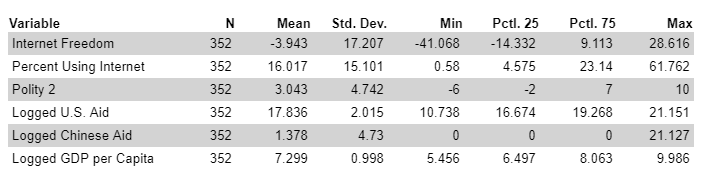
\includegraphics[scale=1.1]{628table2.png}
\end{figure}

A correlation matrix of the variables included in my regressions is given in Figure 2. As can be seen, there are a couple relatively strong relationships between the variables. The variable for regime type, Polity, has a correlation of 0.62 with the internet freedom variable while logged GDP per capita has a correlation of 0.65 with the variable representing the percent of the population using the internet. While possible, I do not think that these correlations are high enough to warrant concerns over multicollinearity or the lack of linear independency in the data. Interestingly, logged U.S. Aid appears somewhat negatively correlated with logged GDP per capita and variable for the percent using the internet is somewhat positively correlated to that for internet freedom. These correlations are relatively small, but it could be interesting to explore the relationship between U.S. aid and GDP.

\pagebreak
\subsubsection*{Figure 2}
\begin{figure}[htbp]
    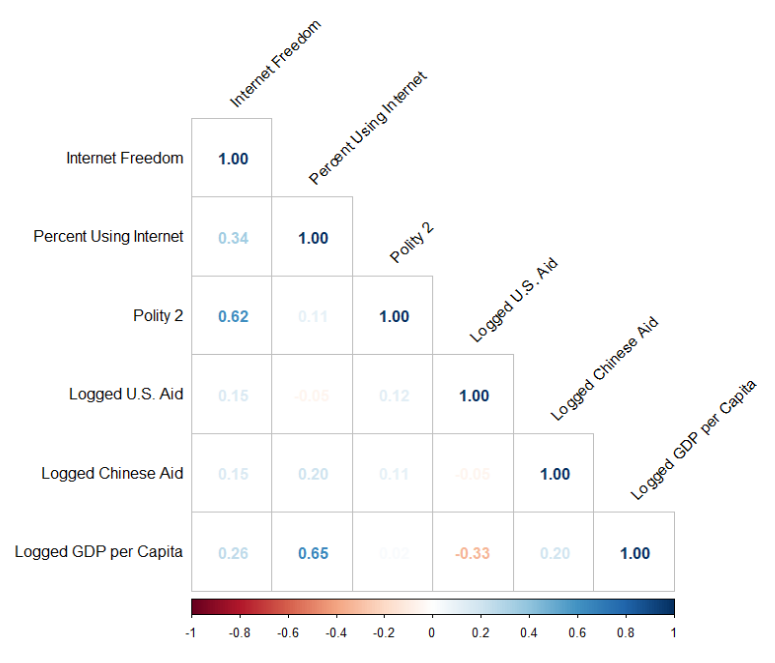
\includegraphics[scale=0.7]{628plot3.png}
\end{figure}

\subsection*{Estimation}
I chose to use ordinary least squares (OLS) for my estimator while employing two-way fixed effects at the country and year level. In choosing fixed effects, I used non-nested model comparison tests that suggested fixed effects to be superior to both no effects and random effects. After testing for heteroskedasticity, I included country-clustered standard errors. 

\pagebreak
\section*{Results}
Table 2 displays regression results from a model with and without an interaction between internet freedom and logged Chinese foreign aid.
\subsection*{Table 2}
\begin{table}[!htbp] \centering 
  \caption*{Logged U.S. Aid and Covariates with Two-way Fixed Effects and Clustered SE's on Country}
  \label{} 
\begin{tabular}{@{\extracolsep{5pt}}lcc} 
\\[-1.8ex]\hline 
\hline \\[-1.8ex] 
 & \multicolumn{2}{c}{Logged U.S. Aid} \\ 
\cline{2-3} 
 & Model 1 & Model 2 \\ 
\hline \\[-1.8ex] 
 Internet Freedom & 0.021$^{***}$ & 0.021$^{***}$ \\ 
  & (0.008) & (0.008) \\ 
  & & \\ 
 Logged Chinese Aid & 0.006$^{*}$ & 0.006$^{*}$ \\ 
  & (0.003) & (0.003) \\ 
  & & \\ 
 Logged GDP per Capita & 0.045 & 0.045 \\ 
  & (0.471) & (0.472) \\ 
  & & \\ 
 Percent Using Internet & $-$0.013 & $-$0.013 \\ 
  & (0.009) & (0.009) \\ 
  & & \\ 
 Polity 2 & 0.004 & 0.004 \\ 
  & (0.031) & (0.031) \\ 
  & & \\ 
 Internet Freedom $\cdot$ Logged Chinese Aid &  & 0.00000 \\ 
  &  & (0.0002) \\ 
  & & \\ 
\hline \\[-1.8ex] 
Observations & 352 & 352 \\ 
R$^{2}$ & 0.038 & 0.038 \\ 
Adjusted R$^{2}$ & $-$0.140 & $-$0.144 \\ 
F Statistic & 2.370$^{**}$ (df = 5; 296) & 1.968$^{*}$ (df = 6; 295) \\ 
\hline 
\hline \\[-1.8ex] 
\textit{Note:}  & \multicolumn{2}{r}{$^{*}$p$<$0.1; $^{**}$p$<$0.05; $^{***}$p$<$0.01} \\ 
\end{tabular} 
\end{table}
\pagebreak

The only covariates that appear statistically significant are the two main explanatory variables. Both internet freedom and logged Chinese aid seem to increase logged U.S. aid on average when accounting for the other covariates. To gauge the substantive size of the coefficients, I plot the marginal effect of internet freedom on logged U.S. aid in Figure 3 and the marginal effect of logged Chinese aid on logged U.S. aid in Figure 4.

Since the effect of internet freedom appears directly related to logged U.S. aid, there is more empirical support for $H_{2a}$, the ``Trickle Down Hypothesis,'' than $H_{2b}$, the ``Bottom up Hypothesis.'' Support for $H_{2a}$ implies that I cannot reject the notion that the U.S. is allocating foreign aid to countries with higher levels of internet freedom.

The ``Intrastate Competition Hypothesis,'' or $H_{1b}$, finds more support than the ``Interstate Competition Hypothesis,'' $H_{1a}$, since logged Chinese aid is directly related to logged U.S. aid. It seems that $H_{1b}$ cannot be rejected, and that the U.S. is plausibly spending more foreign aid in countries where China is also spending more.

Interestingly, there is a lack of support for an interaction between internet freedom and logged Chinese aid. Apparently, the effects of a recipient's internet freedom level and the amount of Chinese aid they are receiving have completely separate effects on U.S. aid. However, it is unclear how consequential this lack of support for the interaction term is, since both variables by themselves are significant and two-way fixed effects are used.

\pagebreak
Figure 3 shows the marginal effect of internet freedom on logged U.S. foreign aid. The coefficient on the internet freedom variable is 0.0206, implying that a one unit increase in a recipient's internet freedom level is associated with an increase in U.S. aid by 2.08 percent on average, accounting for other covariates. This appears to be a substantively large effect.

\subsection*{Figure 3}
\begin{figure}[htbp]
    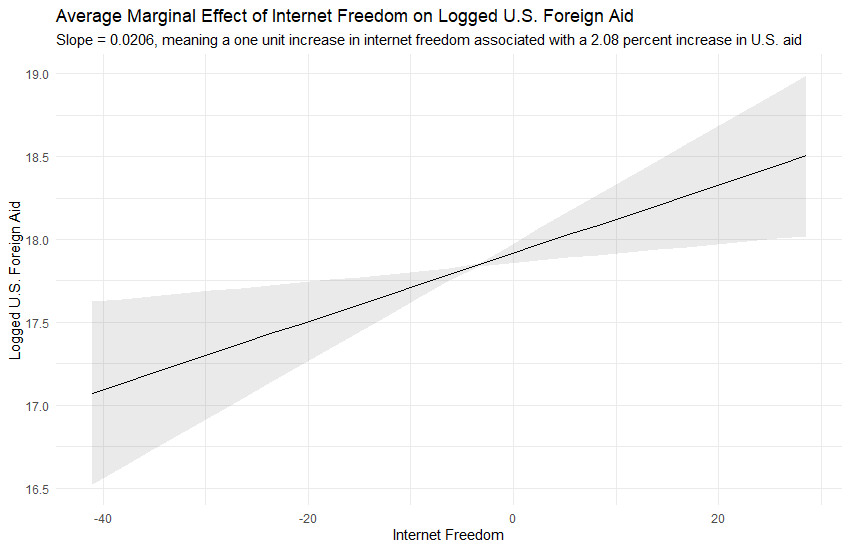
\includegraphics[scale=0.7]{628plot1.png}
\end{figure}

\pagebreak
Figure 4 graphs the marginal effect of logged Chinese foreign aid on logged U.S. foreign aid. The coefficient on the variable for logged Chinese foreign aid is 0.0058, implying that a one percent increase in Chinese aid is associated with a 0.0058 percent increase in U.S. aid on average, accounting for other covariates. This does not appear to be a substantively large effect.

\subsection*{Figure 4}
\begin{figure}[htbp]
    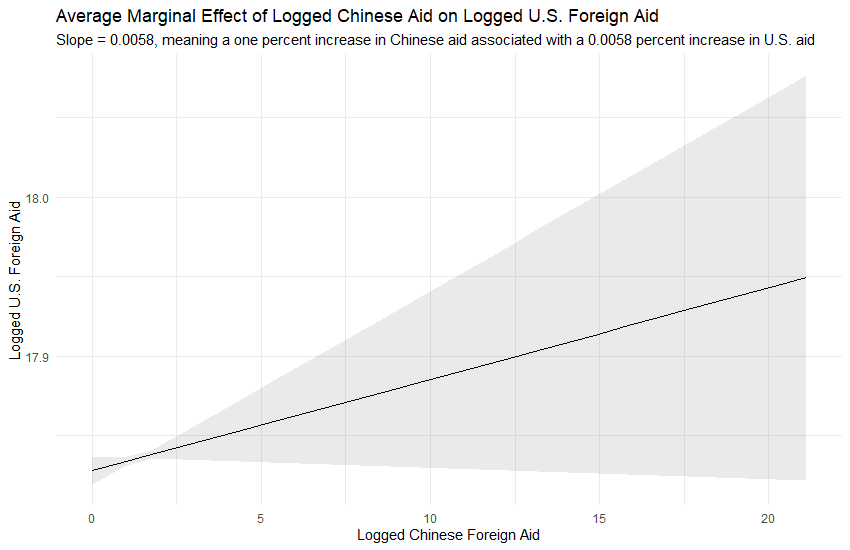
\includegraphics[scale=0.7]{628plot2.png}
\end{figure}
\pagebreak 

\section*{Discussion}
The support found for both $H_{1b}$ and $H_{2a}$ is a little surprising for the following reason. While it appears that the direct relationship between internet freedom and U.S. aid is in accordance with the literature ($H_{2a}$), this relationship was hypothetically built on the previous finding that U.S. aid is relatively ineffective in countries receiving Chinese aid (\cite{dreher2021}). 

Subsequently, it should also be the case that U.S. aid is inversely related to Chinese aid ($H_{1a}$) if the U.S. rationally desires its aid to be effective, which should mean that aid would be going to countries with more liberal internet systems due to the absence of illiberal effects from Chinese aid. However, U.S. aid seems to also be directly related to Chinese aid, undermining this logic. Thus, it seems that the U.S. either does not highly value the effectiveness of its aid or that its aid is more effective at improving internet liberalism where China is also spending money.

Regardless, it is interesting that some support was found for both the ``Trickle Down Hypothesis'' and the ``Intrastate Competition Hypothesis.'' Given the lack of an interaction term, it would seem that the U.S. is reacting to the influx of Chinese aid by increasing foreign aid spending in countries where either Chinese aid is also present or the recipient has a relatively liberal internet model, but not both. Further investigation of this phenomenon in the data is required.

\section*{Conclusion}
In this article I argue that it is rational for the U.S. to respond to a global increase in Chinese foreign aid by changing its own aid allocation strategy and focusing on how recipients treat the internet. In particular, the literature seems to imply that the U.S. should concentrate spending in countries devoid of Chinese aid and with highly liberal models of internet governance.

Analyzing 44 African countries from 2010-2017, I find mixed results for this set of expectations. While U.S. aid indeed seems positively related to a measure of internet governance, it is also directly related to Chinese foreign aid.

Given these findings, I suggest two future lines of research on this topic. Firstly, more rigorous research needs to be conducted on the true relationship between China's aid projects and the effects on internet governance. Much of the existing discussion on this area is non-scientific and biased towards U.S. interests. The results shown here do not directly speak to how Chinese foreign aid affects recipient internet usage, but there was a lack of support for the hypothesis that U.S. aid and Chinese aid should be inversely related ($H_{1a}$). Perhaps these countries do not have entirely opposite, neatly ideological goals concerning how countries use the internet around the world.

Secondly, depending on the strength of these results, there should be further work done explicating why exactly the U.S. is interested in boosting internet liberalism in Africa. If the U.S. is truly interested in increasing democracy and liberalism around the world in general, it is unclear if this motivation is sufficient to account for such large expenditures if the U.S. is a rational actor. In other words, to the extent that the internet is relevant for the foreign aid decision of the U.S., it is worthwhile pursuing explanations for what the U.S. materially gains from this practice.

\pagebreak
\section*{Appendix}
The entry game described in the theory section (Figure 1) is solved via backwards induction. The parameter $\delta$ inversely represents the influence that U.S. aid has on a recipient's internet model while $\gamma$ inversely represents the influence of Chinese aid. In other words, low values of $\delta$ or $\gamma$ imply high degrees of influence. 

Hypothetically, if $China$ chooses to $Spend$, the $U.S.$ chooses to $Spend$ if and only if (iff):

\begin{tabular}{c l}
    $\frac{\gamma}{\delta}-c_2> \delta$ &  As $\delta$ increases, this condition becomes harder to satisfy.\\
\end{tabular}

Hypothetically, if $China$ chooses to $\neg Spend$, the $U.S.$ chooses to $Spend$ iff:

\begin{tabular}{c l}
    $\frac{1}{\delta}-c_2> \delta$ &  As $\delta$ increases, this condition becomes harder to satisfy.\\
\end{tabular}

Hypothetically, when $\delta$ is arbitrarily small, the $U.S.$ chooses to $Spend$ and $China$ $Spend$s iff:

\begin{tabular}{c l}
    $\frac{\delta}{\gamma}-c_1> \gamma$ &  As $\gamma$ increases, this condition becomes harder to satisfy.\\
\end{tabular}

Hypothetically, when $\delta$ is arbitrarily large, the $U.S.$ chooses to $\neg Spend$ and $China$ $Spend$s iff:

\begin{tabular}{c l}
    $\frac{1}{\gamma}-c_1> \gamma$ &  As $\gamma$ increases, this condition becomes harder to satisfy.\\
\end{tabular}

Summarily, if $\delta$ and $\gamma$ are arbitrarily small, both players will $Spend$. When $\delta$ is arbitrarily small and $\gamma$ is arbitrarily large, the $U.S.$ $Spend$s and $China$ $\neg Spend$. If $\delta$ is arbitrarily large and $\gamma$ is arbitrarily small, the $U.S.$ $\neg Spend$ and $China$ $Spend$s. When $\delta$ is arbitrarily large and $\gamma$ is arbitrarily large, neither player $Spend$s.

\nocite{mechkova2022a}
\nocite{pemstein2022}
\nocite{coppedge2022}
\nocite{coppedge2022a}
\nocite{coppedge2022b}
\nocite{coppedge2022c}
\nocite{coppedge2022d}
\pagebreak
\printbibliography
\end{document}